\documentclass[crop,tikz]{standalone}


\begin{document}
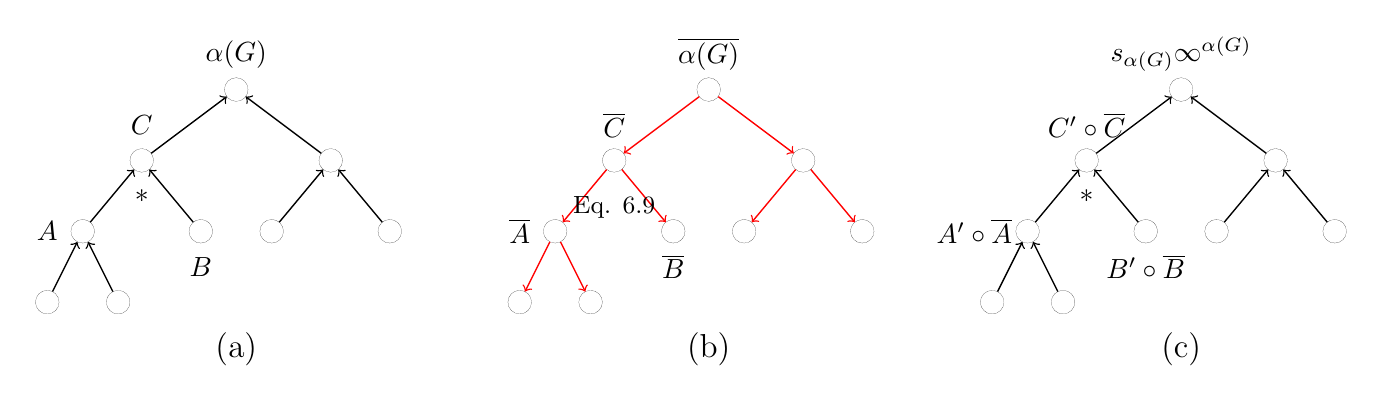
\begin{tikzpicture}[scale=1.5]
\node[circle, inner sep=0cm, draw=black, line width=0.03, fill=none, minimum size=0.3cm] at (0.0, 0.0) (1234) {};
\node[circle, inner sep=0cm, draw=black, line width=0.03, fill=none, minimum size=0.3cm] at (-0.8, -0.6) (1235) {};
\node[circle, inner sep=0cm, draw=black, line width=0.03, fill=none, minimum size=0.3cm] at (0.8, -0.6) (1236) {};
\node[circle, inner sep=0cm, draw=black, line width=0.03, fill=none, minimum size=0.3cm] at (-1.3, -1.2) (1237) {};
\node[circle, inner sep=0cm, draw=black, line width=0.03, fill=none, minimum size=0.3cm] at (-0.30000000000000004, -1.2) (1238) {};
\node[circle, inner sep=0cm, draw=black, line width=0.03, fill=none, minimum size=0.3cm] at (1.3, -1.2) (1239) {};
\node[circle, inner sep=0cm, draw=black, line width=0.03, fill=none, minimum size=0.3cm] at (0.30000000000000004, -1.2) (1240) {};
\node[circle, inner sep=0cm, draw=black, line width=0.03, fill=none, minimum size=0.3cm] at (-1.6, -1.8) (1241) {};
\node[circle, inner sep=0cm, draw=black, line width=0.03, fill=none, minimum size=0.3cm] at (-1.0, -1.8) (1242) {};
\draw[<-, line width=0.5pt] (1234) -- (1235);
\draw[<-, line width=0.5pt] (1234) -- (1236);
\draw[<-, line width=0.5pt] (1235) -- (1237);
\draw[<-, line width=0.5pt] (1235) -- (1238);
\draw[<-, line width=0.5pt] (1236) -- (1239);
\draw[<-, line width=0.5pt] (1236) -- (1240);
\draw[<-, line width=0.5pt] (1237) -- (1241);
\draw[<-, line width=0.5pt] (1237) -- (1242);
\node[] at (0.0, 0.3) {$\alpha(G)$};
\node[] at (-1.6, -1.2) {$A$};
\node[] at (-0.30000000000000004, -1.5) {$B$};
\node[] at (-0.8, -0.3) {$C$};
\node[] at (-0.8, -0.8999999999999999) {$*$};
\node[] at (0.0, -2.2) {\large (a)};
\node[circle, inner sep=0cm, draw=black, line width=0.03, fill=none, minimum size=0.3cm] at (4.0, 0.0) (1243) {};
\node[circle, inner sep=0cm, draw=black, line width=0.03, fill=none, minimum size=0.3cm] at (3.2, -0.6) (1244) {};
\node[circle, inner sep=0cm, draw=black, line width=0.03, fill=none, minimum size=0.3cm] at (4.8, -0.6) (1245) {};
\node[circle, inner sep=0cm, draw=black, line width=0.03, fill=none, minimum size=0.3cm] at (2.7, -1.2) (1246) {};
\node[circle, inner sep=0cm, draw=black, line width=0.03, fill=none, minimum size=0.3cm] at (3.7, -1.2) (1247) {};
\node[circle, inner sep=0cm, draw=black, line width=0.03, fill=none, minimum size=0.3cm] at (5.3, -1.2) (1248) {};
\node[circle, inner sep=0cm, draw=black, line width=0.03, fill=none, minimum size=0.3cm] at (4.3, -1.2) (1249) {};
\node[circle, inner sep=0cm, draw=black, line width=0.03, fill=none, minimum size=0.3cm] at (2.4, -1.8) (1250) {};
\node[circle, inner sep=0cm, draw=black, line width=0.03, fill=none, minimum size=0.3cm] at (3.0, -1.8) (1251) {};
\draw[->, draw=red, line width=0.5pt] (1243) -- (1244);
\draw[->, draw=red, line width=0.5pt] (1243) -- (1245);
\draw[->, draw=red, line width=0.5pt] (1244) -- (1246);
\draw[->, draw=red, line width=0.5pt] (1244) -- (1247);
\draw[->, draw=red, line width=0.5pt] (1245) -- (1248);
\draw[->, draw=red, line width=0.5pt] (1245) -- (1249);
\draw[->, draw=red, line width=0.5pt] (1246) -- (1250);
\draw[->, draw=red, line width=0.5pt] (1246) -- (1251);
\node[] at (4.0, 0.3) {$\overline{\alpha(G)}$};
\node[] at (2.4000000000000004, -1.2) {$\overline{A}$};
\node[] at (3.7, -1.5) {$\overline{B}$};
\node[] at (3.2, -0.3) {$\overline{C}$};
\node[] at (3.2, -1.0) {\small Eq. 6.9};
\node[] at (4.0, -2.2) {\large (b)};
\node[circle, inner sep=0cm, draw=black, line width=0.03, fill=none, minimum size=0.3cm] at (8.0, 0.0) (1252) {};
\node[circle, inner sep=0cm, draw=black, line width=0.03, fill=none, minimum size=0.3cm] at (7.2, -0.6) (1253) {};
\node[circle, inner sep=0cm, draw=black, line width=0.03, fill=none, minimum size=0.3cm] at (8.8, -0.6) (1254) {};
\node[circle, inner sep=0cm, draw=black, line width=0.03, fill=none, minimum size=0.3cm] at (6.7, -1.2) (1255) {};
\node[circle, inner sep=0cm, draw=black, line width=0.03, fill=none, minimum size=0.3cm] at (7.7, -1.2) (1256) {};
\node[circle, inner sep=0cm, draw=black, line width=0.03, fill=none, minimum size=0.3cm] at (9.3, -1.2) (1257) {};
\node[circle, inner sep=0cm, draw=black, line width=0.03, fill=none, minimum size=0.3cm] at (8.3, -1.2) (1258) {};
\node[circle, inner sep=0cm, draw=black, line width=0.03, fill=none, minimum size=0.3cm] at (6.4, -1.8) (1259) {};
\node[circle, inner sep=0cm, draw=black, line width=0.03, fill=none, minimum size=0.3cm] at (7.0, -1.8) (1260) {};
\draw[<-, draw=black, line width=0.5pt] (1252) -- (1253);
\draw[<-, draw=black, line width=0.5pt] (1252) -- (1254);
\draw[<-, draw=black, line width=0.5pt] (1253) -- (1255);
\draw[<-, draw=black, line width=0.5pt] (1253) -- (1256);
\draw[<-, draw=black, line width=0.5pt] (1254) -- (1257);
\draw[<-, draw=black, line width=0.5pt] (1254) -- (1258);
\draw[<-, draw=black, line width=0.5pt] (1255) -- (1259);
\draw[<-, draw=black, line width=0.5pt] (1255) -- (1260);
\node[] at (8.0, 0.3) {$s_{\alpha(G)}\infty^{\alpha(G)}$};
\node[] at (6.25, -1.2) {$A'\circ\overline{A}$};
\node[] at (7.7, -1.5) {$B'\circ\overline{B}$};
\node[] at (7.2, -0.3) {$C'\circ\overline{C}$};
\node[] at (7.2, -0.8999999999999999) {$*$};
\node[] at (8.0, -2.2) {\large (c)};
\end{tikzpicture}
\end{document}
